\chapter{Návrh}

Tato kapitola popisuje návrh implementace a komplementárních struktur.

\section{Toolbar}

Toolbar je strukturová komponenta, která obsahuje skupinu focusovatelných elementů.

\begin{figure}[htp]
    \centering
    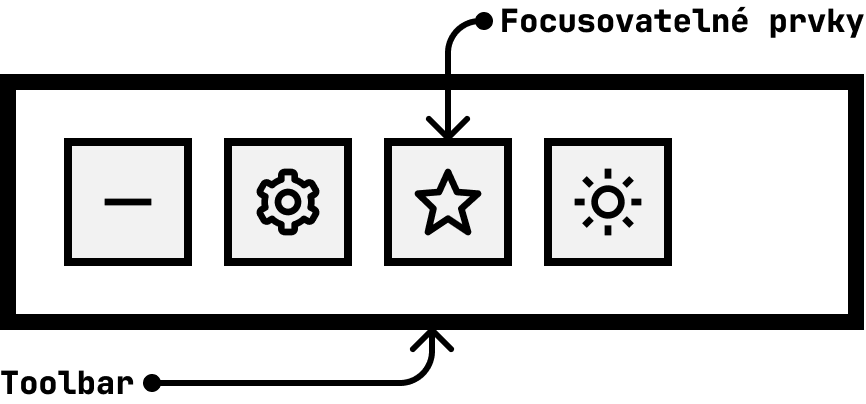
\includegraphics[max size={\linewidth}{\textheight}]{./assets/figures/anatomy/toolbar.png}
    \captionsetup{justification=centering}
    \caption{Anatomie komponenty Toolbar}
\end{figure}

Hlavní přínos této komponenty je jednodušší klávesová navigace pomocí klávesových šipek a dalších zkratek namísto klasického proklikávání tabulátorem.

Pro splnění požadavku \hyperref[ofr11]{\fr{OFR 1.1}} je potřeba splnit následující podmínky:

\begin{enumerate}
    \item Tabulátor směrem dopředu skočí na první, nebo naposled vybraný focusovatelný prvek v rámci Toolbaru.
    \item Tabulátor směrem dopředu, když je focus v rámci Toolbaru, skočí na první focusovatelný prvek mimo Toolbar.
    \item Šipky vlevo a vpravo přesunou focus mezi focusovatelnými prvky v rámci Toolbaru pokud je orientace toolbaru horizontální.
    \item Šipky nahoru a dolů přesunou focus mezi focusovatelnými prvky v rámci Toolbaru pokud je orientace toolbaru vertikální.
    \item Klávesy \texttt{Home} a \texttt{End} přesunou focus na první, respektive poslední focusovatelný prvek v rámci Toolbaru.
\end{enumerate}

\section{SpinButton}

SpinButton je formulářová komponenta, která vymezuje rozsah diskrétních hodnot a typicky umožňuje uživateli změnit její hodnotu pomocí navyšovacích a snižovacích tlačítek, nebo alternativně skrze textový vstup.

\begin{figure}[htp]
    \centering
    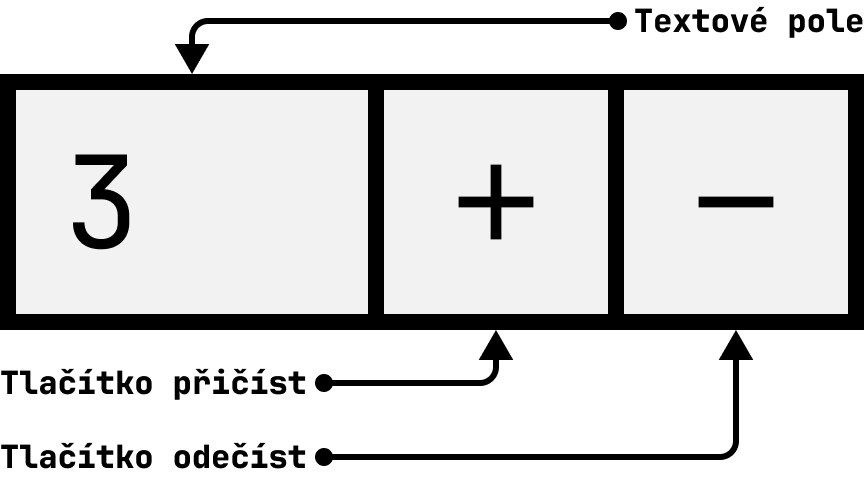
\includegraphics[max size={\linewidth}{\textheight}]{./assets/figures/anatomy/spinbutton.png}
    \captionsetup{justification=centering}
    \caption{Anatomie komponenty SpinButton}
\end{figure}

\section{Carousel}

Carousel je komponenta pro zobrazení multimediálního obsahu v podobě obrázků, videí nebo alternativních prvků.
V rámci \gls{apg} jsou popsané tři varianty této komponenty popsané níže.

\begin{figure}[htp]
    \centering
    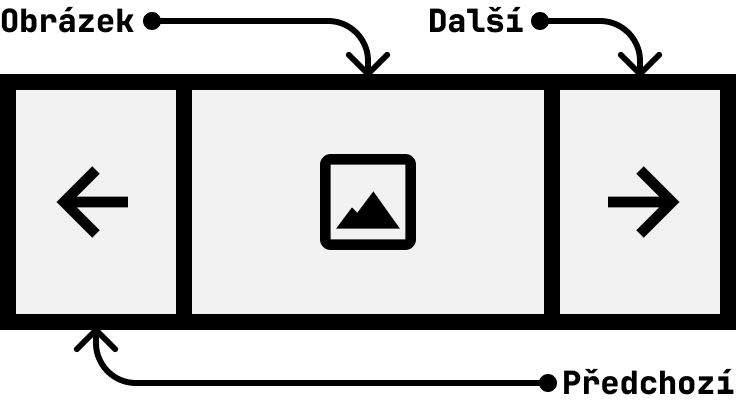
\includegraphics[max size={\linewidth}{\textheight}]{./assets/figures/anatomy/carousel.png}
    \captionsetup{justification=centering}
    \caption{Anatomie komponenty Carousel}
\end{figure}

\subsection{Basic Carousel}

TODO

\subsection{Tabbed Carousel}

TODO

\subsection{Grouped Carousel}

TODO
